% 1.5 page
% I have a lot to illustrate, these are for me to understand the system better

\subsection{AV Perception System}

In the state-of-art AV systems, perception plays an important role in ensuring the safety. 
The sensors are used to detect the obstacles and measure the velocity or distance in real time. 
Typical systems in high-level, such as Level 4\cite{level4} AVs adopt both LiDAR and camera for visual perception.
LiDAR\cite{lidar} can detect the ranges by shooting an object with a laser and measure the distance by getting the time for the light to be reflected back to the receiver.
Compared with RADAR, LiDAR is much more accurate in resolution.
Thus it's used to reconstruct exact 3D models of objects in autonomous systems.
However, it's difficult to get the texture-related information such as the color\cite{lidar-text}. 
On the other hand, camera images are good at providing shape and texture information, but lack depth and distance information due to its 2D imaging.
In order to compensate the weaknesses and utilize the strength in each sensor, most AV systems will adopt Multi-Sensor Fusion(MSF) design, 
in which it will fuse the sensor reading from both LiDAR and camera.

Figure~\ref{fig:module} shows an overview of the perception module in common AV system\cite{apollo}.
3D objects are first perceived by LiDAR and camera to generate point clouds(LiDAR) and frames of images(camera).
These raw sensor output will then go through a pre-processing unit for the aggregated feature and ROI(Region of Interest) extraction.
Pre-processed features will be fed into the LiDAR perception network and camera perception network respectively to get the detection results.
The MSF algorithm will fuse the outputs of two perception networks and give the final detection output.

In this project, we focus on the camera perception part. 
3D objects are sensed by the camera in the form of 2D images. 
When a random obstacle in put in the middle of the road, a synthesized image with obstacle and road background is generated.
This image will then be fed into the object detection neural network for results.

\subsection{Synthesized Scene}

In order to synthesize the obstacle with the road background, many prior works\cite{msf-adv} use Neural 3D Mesh Renderer(NMR) for camera rendering\cite{nmr}.
NMR provides a way to generate a 2D image from the 3D world. 
It can transfer rendering gradient with consideration of texture, lighting, camera and the object shapes.
Given the camera pose, light condition, relative position between the camera and the overall background, 
NMR will provide the image output of this background with certain camera setting. 

Fig. \ref{fig:synthe} overviews the image synthesizing process in MSF-ADV\cite{msf-adv}.
It first chooses the background from the target road, and the obstacle that it intends to put on the road, for example, a brown chair.
The 3D chair is presented in the form of point cloud, which is a set of data points in space.
Camera parameters and light condition will be set to rendering this chair to a 2D image. 
Then the relative location of the chair in the background is set. 
Original pixels in the background will be masked by the pixels in the 2D chair image to simulate how chair is put in the middle of the road.
Before feeding the synthesized scene into detection neural networks, some pre-processing steps such as data transformation,
utilizing the Region of Interest(RoI) filter to clear unrelated input parts and collecting aggregated features are performed.
These pre-processing processes can reduce the input size fed into the neural network and greatly improve the inference speed.

In this project, we will use this as the target pipeline for generating synthesized scene and will evaluate the authenticity of the synthesized output.

% camera rendering theory
% sample synthesized scene & pipeline 

\subsection{Adversarial 3D Object Attacks}

Prior works find that it's easy to fool models with deceptive data, which causes the malfunction in the neural network model.
This kind of adversarial attacks are also studied in the context of physical world\cite{adv1, adv2, adv3}.
In the AV systems, some prior works proposed physical adversarial attacks by placing obstacles in the air or on the road\cite{adv1, adv2, adv3}.
Some are targeting at fooling the camera-based perception neural network\cite{adv1, adv2, adv3} while others are focusing on LiDAR-based perception neural network\cite{lidar1, 6}.
Recently, considering that MSF design is widely used in AD systems, MSF-ADV\cite{msf-adv} is proposed to attack both LiDAR and camera sensors with a 3D adversarial object.

MSF-ADV\cite{msf-adv} treats the process of generating the adversarial attacks as an optimization problem and Fig. \ref{fig:attack-pipe} provides an overview of the process to generate adversarial obstacles. 
It first picks a normal 3D object and apply 3D transformations including rotation, position shifting to get different angles of the object.
This is to improve the robustness of the obstacle in various kinds of environment.
Then it will generate point cloud and image of this 3D object through ray-tracing\cite{ray-tracing} and NMR\cite{nmr} to simulate the perception output of LiDAR and camera sensors.
These two sensor outputs will be integrated with the road background and pre-processed before being sent to perspective perception neural networks and MSF algorithm.
The attacker is assumed to be able to perturb the shape and position of the 3D object.
Also, adversarial loss function is designed to cause the malicious object not to be detected by MSF algorithm as well as keep the obstacle stealthy.
After obtaining the generated malicious object, the attacker can just 3D print it and place it in the road according to the parameters in the optimization process.

In this project, we will use MSF-ADV\cite{msf-adv} as the target adversarial attack in the evaluation part.
MSF-ADV\cite{msf-adv} uses the same method in previous section to generate synthesized scene. 
Therefore, we want to see whether the authenticity of the synthesized scene will influence the effectiveness of the generated malicious object.



%\subsection{Point cloud}
%
%Point cloud refers to a set of data points in space to represent a 3D object produced by a 3D scanner. 
%As 3D data can provide a better understanding of the shape and geometric information in the surrounding environment\cite{point-cloud-survey},
%AV systems are usually equipped with LiDAR sensors to generate the 3D point cloud.
%However, unlike 2D images, the 3D point cloud is highly unstructured and difficult to interpret.
%For example, traditional 2D image filtering techniques like mean filtering\cite{mean-filter} and median filtering\cite{median-filter} can't be applied on the 3D point cloud.
%And previous 2D image neural networks are also not applicable.
%This makes the 3D point cloud smoothing and object reconstruction more difficult.
%
%\subsection{LiDAR perception in AV}
%
%\textbf{ADD FIGURE!}
%Figure~\ref{fig:module} shows the perception module in common AV system\cite{apollo}.
%3D objects are first perceived by LiDAR and camera to generate point clouds(LiDAR) and frames of images(camera).
%These sensor data then go through a pre-processing unit to extract some aggregated features and ROI(Region of Interest).
%Pre-processed data will be fed into the LiDAR perception network and camera perception network respectively in the MSF algorithm unit.
%The MSF algorithm will fuse the outputs of two perception networks and give the detection output.
%
%In this project, we plan to add point cloud recovery between the LiDAR rendering part and pre-processing part,
%given the fact that the MSF algorithm can produce correct results with at least one correct sensor output.
%% system structure
%------------------------
%\begin{figure}
%	\centering
%	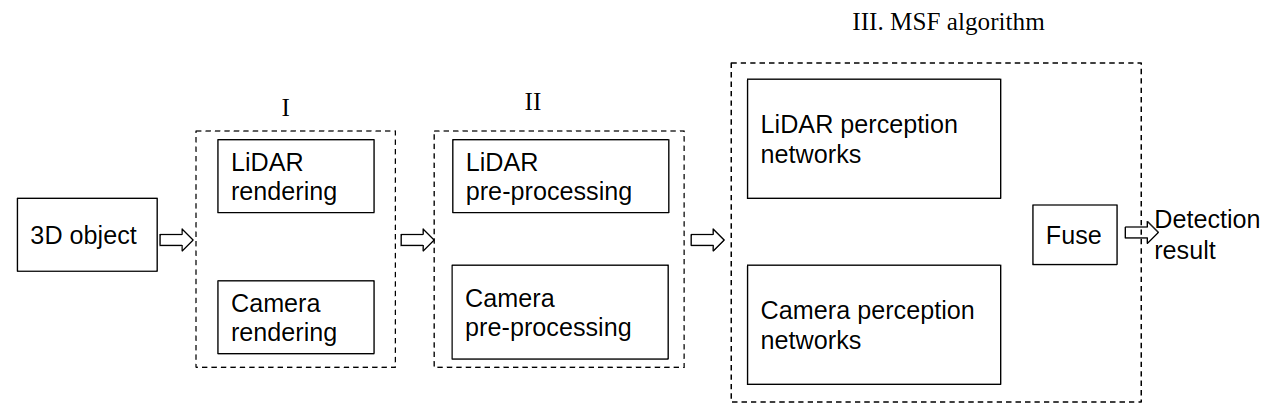
\includegraphics[width=0.8\linewidth]{figure/structure.png}
%	\caption{Perception module in AV systems}
%	\label{fig:module}
%\end{figure}
%
%\begin{figure}
%	\centering
%	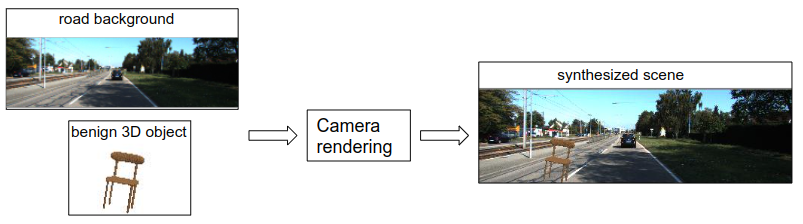
\includegraphics[width=0.8\linewidth]{figure/synthesized.png}
%	\caption{Synthesized scene through camera rendering}
%	\label{fig:synthe}
%\end{figure}
%
%\begin{figure}
%	\centering
%	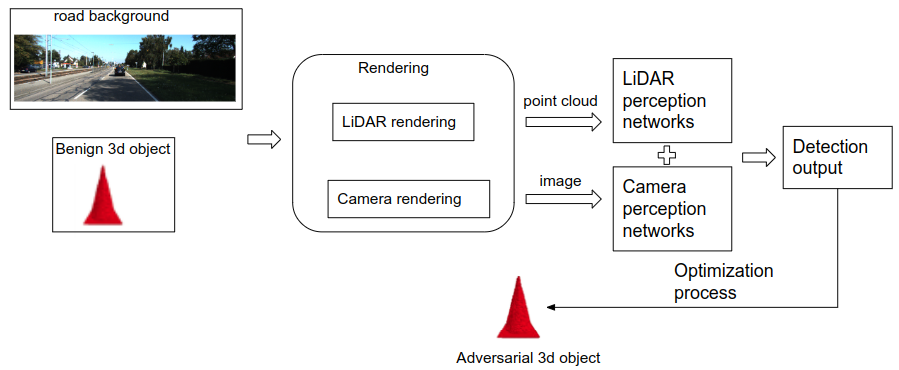
\includegraphics[width=0.8\linewidth]{figure/attack-pipeline.png}
%	\caption{Pipeline for generating adversarial 3D object attacks for both Lidar and Camera}
%	\label{fig:attack-pipe}
%\end{figure}
%------------------------
